\chapter{Fallstudie: Verteiltes Legacy-System}
\label{ch:fallstudie}

Als Fallstudie betrachtet diese Masterarbeit das in~\citep{liebig_2025_architectural_refactoring} untersuchte verteilte Legacy-System \textit{\enquote{\gls{marc}}}~\footnote{Das reale \gls{marc} umfasst mehr als 30 Komponenten; in dieser Masterarbeit wird eine für die Analyse reduzierte Sicht auf die relevanten Kommunikations- und Servicepfade verwendet.} der Firma GS electronic Gebr. Schönweitz GmbH~\citep{gselectronic}. \gls{marc} ist ein verteiltes Alarmempfangssystem, das externe Alarmanlagen überwacht sowie Alarmmeldungen empfängt, verarbeitet und in einer Datenbank persistiert, um sie für die anschließende Bearbeitung durch Mitarbeiter in einer Leitstelle bereitzustellen. Abbildung~\ref{fig:marc-simple-architektur} zeigt eine vereinfachte Architektur von \gls{marc} sowie seine zentrale Komponente \textit{\enquote{\gls{ars}}} zur Verarbeitung von Alarmmeldungen. Ist \gls{ars} nicht verfügbar, können keine Alarmmeldungen bearbeitet werden.

\begin{figure}[H]
    \centering
    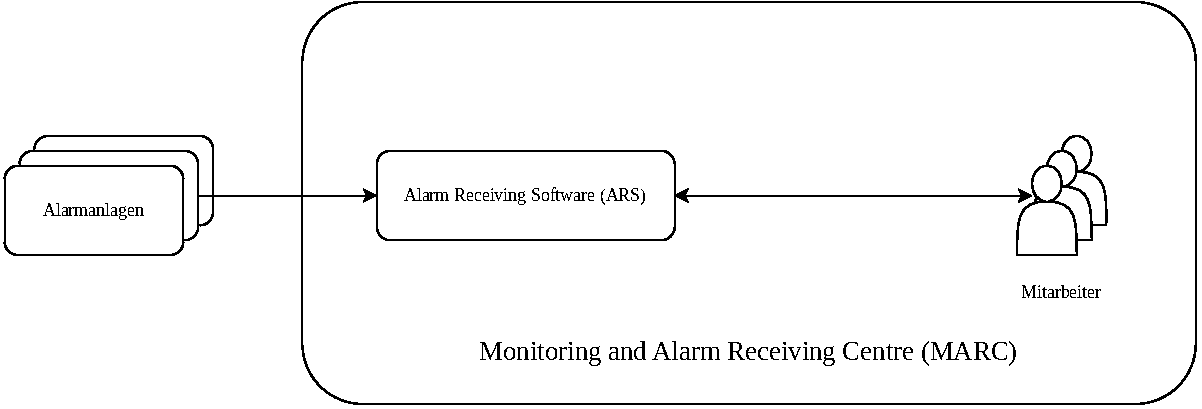
\includegraphics[width=\textwidth]{./img/drawio/marc_simple.pdf}
    \caption{Vereinfachte Gesamtarchitektur des Legacy-Systems \acrshort{marc}.}
    \label{fig:marc-simple-architektur}
\end{figure}

\section{Architektur}
\label{sec:marc-architektur}

Wie im vorherigen Abschnitt beschrieben, bildet die \gls{ars} die zentrale Komponente des \gls{marc}-Systems. Ihre Hauptaufgabe besteht darin, eingehende Alarmmeldungen zu empfangen, zu verarbeiten und in einer Datenbank zu persistieren. Intern setzt sich die \gls{ars} aus mehreren Services zusammen, die im Folgenden als \gls{srv}~1, \gls{srv}~2 und \gls{srv}~3 bezeichnet werden~\ref{fig:ars-architektur}. \gls{srv}~1 stellt dabei die primäre \gls{http}-Schnittstelle bereit, über die Alarmmeldungen von den externen Alarmanlagen entgegengenommen werden. Nach dem Empfang einer Alarmmeldung durchläuft sie eine synchrone \textit{Request-Response-Kette}~\footnote{Request-Response-Kette bezeichnet eine sequentielle Folge synchroner Request-Response-Interaktionen über mehrere Services, bei der jeder nachgelagerte Schritt erst nach erfolgreicher Antwort des vorherigen Schritts fortgesetzt wird.} über alle beteiligten Services bis hin zu \gls{srv}~3, welcher die finale Verarbeitung und die Persistierung der Alarmmeldung in einer Datenbank übernimmt. Die Kommunikation innerhalb dieser Kette erfolgt über eine Kombination aus \gls{http}-Requests und einem proprietären \gls{tcp}-Protokoll. Erst nachdem \gls{srv}~3 die Verarbeitung der Alarmmeldung erfolgreich abgeschlossen hat, wird eine Bestätigung über die VerarbeitungsKette an die sendende Alarmanlage zurückgeleitet. Die Antworten der einzelnen Services dienen ausschließlich als Bestätigung des erfolgreichen Empfangs beziehungsweise der erfolgreichen Verarbeitung und enthalten keine zusätzlichen Nutzdaten. Bei negativen Antworten, Netzstörungen oder Timeouts senden die Alarmanlagen die Alarmmeldungen erneut. Abbildung~\ref{fig:ars-architektur} veranschaulicht die interne Verarbeitungskette der \gls{ars}. Eine eingehende Alarmmeldung wird von \gls{srv}~1 angenommen, synchron über \gls{srv}~2 an \gls{srv}~3 weitergereicht und erst nach erfolgreicher Verarbeitung bestätigt.

\begin{figure}[H]
    \centering
    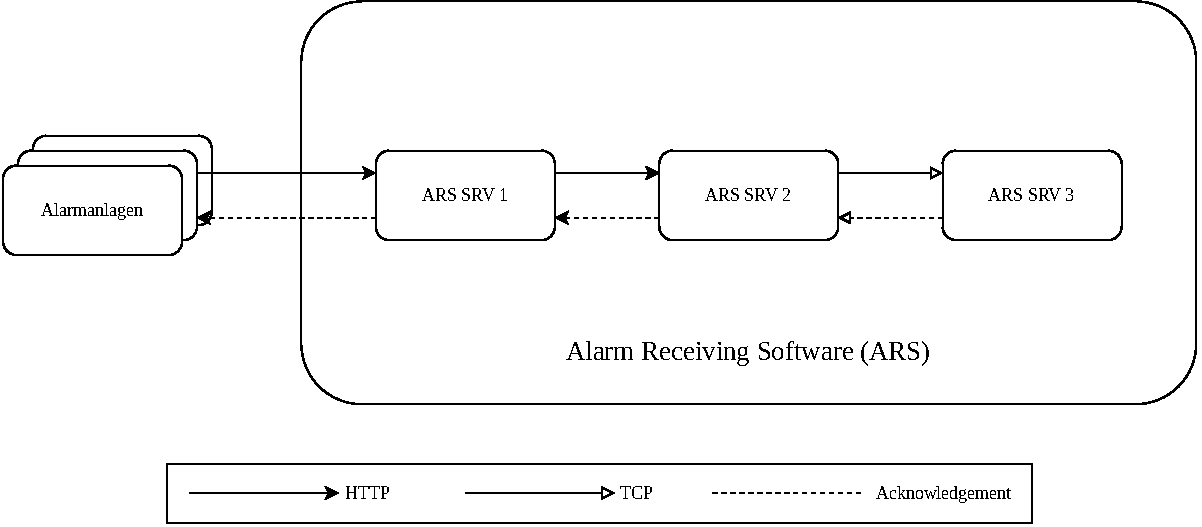
\includegraphics[width=\textwidth]{./img/drawio/ars.pdf}
    \caption{Interne Service-Architektur der Alarm Receiving Software (\acrshort{ars}).}
    \label{fig:ars-architektur}
\end{figure}

\gls{marc} ist über drei Rechenzentren repliziert, wobei in jedem Replikat eine eigene Instanz von \gls{ars} betrieben wird. Während die Services \gls{srv}~1 und \gls{srv}~2 in allen \gls{ars}-Instanzen zur Lastverteilung im Aktiv-Aktiv-Modus operieren, ist \gls{srv}~3 im Aktiv-Passiv-Modus ausgelegt. Folglich ist zu jedem Zeitpunkt nur eine Instanz von \gls{srv}~3 aktiv und für die Verarbeitung von Alarmmeldungen zuständig. Abbildung~\ref{fig:marc-architektur} zeigt die replizierte \gls{marc}-Architektur über drei Rechenzentren und wie die verschiedenen Services miteinander interagieren.

\begin{figure}[H]
    \centering
    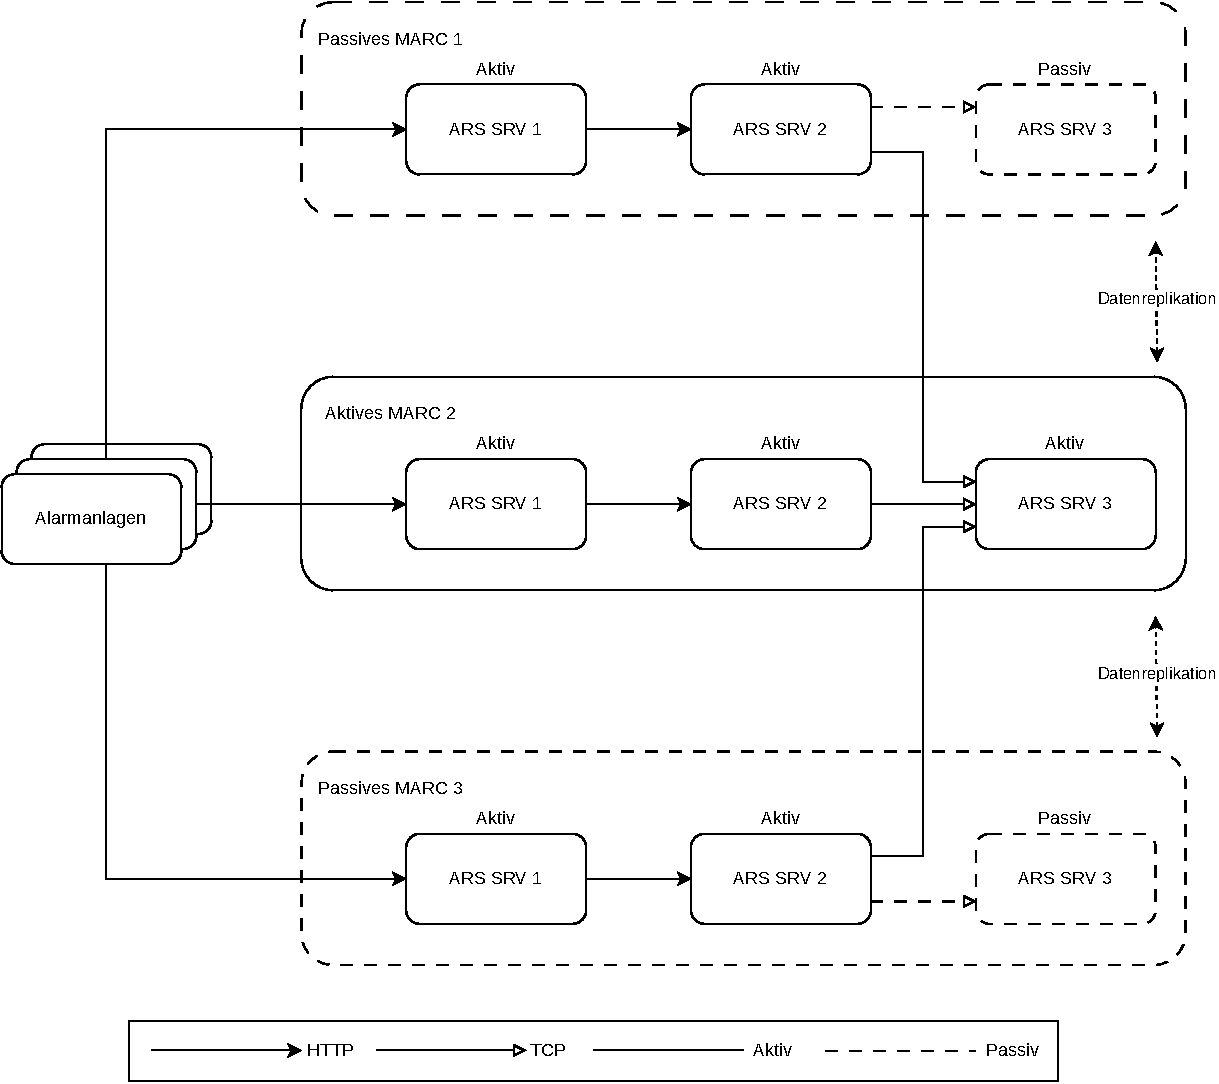
\includegraphics[width=\textwidth]{./img/drawio/marc.pdf}
    \caption{Replizierte \acrshort{marc}-Architektur über drei Rechenzentren mit Aktiv-Aktiv- und Aktiv-Passiv-Betrieb.}
    \label{fig:marc-architektur}
\end{figure}

\section{Design Smells im Legacy-System}
\label{sec:design-smells}

Die Architektur von \gls{marc} führt laut~\citep{liebig_2025_architectural_refactoring} zu mehreren strukturellen Problemen. Die Analyse von~\citep{liebig_2025_architectural_refactoring} identifiziert diese strukturellen Problemen und klassifiziert sie in die folgenden Design Smells:

\begin{itemize}
    \item \textbf{Smell~1}: \textit{Synchrone Request-Response-Ketten}. Die sequentielle Kopplung der \gls{ars}-Services; \gls{srv}~1, \gls{srv}~2 und \gls{srv}~3 führt zu einer Akkumulation der Latenzen. Die Gesamtantwortzeit der Verarbeitung einer Alarmmeldung ergibt sich aus der Summe der Latenzen der Einzelkomponenten.

    \item \textbf{Smell~2}: \textit{Heterogene Redundanzmodi}. Der parallele Einsatz von Aktiv-Aktiv für die \gls{ars}-Services; \gls{srv}~1 und \gls{srv}~2 sowie Aktiv-Passiv für \gls{srv}~3 innerhalb derselben Verarbeitungskette verursacht einen Flaschenhals. Dadurch wird der Gesamtdurchsatz des Systems auf die Kapazität einer einzelnen aktiven \gls{srv}~3-Instanz begrenzt.

    \item \textbf{Smell~3}: \textit{Manuelles Ausfall-Management}. Das System kann Ausfälle nicht autonom beheben, sondern erfordert eine manuelle Überwachung und Intervention durch Mitarbeiter. Dieser manuelle Arbeitsschritt dauert oft Minuten, während Sicherheitsnormen wie die \textit{EN 50136}~\citep{din_en_50136-12012-08_alarm_2012} Reaktionen innerhalb weniger Sekunden fordern. Dadurch ist das System im Ernstfall zu langsam und fehleranfällig.

    \item \textbf{Smell~4}: \textit{Abhängigkeit von Exactly-Once-Delivery}. Das System ist auf eine \textit{Exactly-Once-Delivery} angewiesen, da der Verarbeitung von Alarmmeldungen die \textit{Idempotenz}~\footnote{Idempotenz bedeutet, dass eine Operation beliebig oft wiederholt werden kann, ohne dass sich der Systemzustand nach der ersten erfolgreichen Anwendung ändert~\citep{helland2012idempotence}.} fehlt. Das bedeutet intuitiv, dass das System nicht nativ mit Duplikaten umgehen kann, die durch wiederholte Übertragungen der Alarmanlagen entstehen. Mitarbeiter in der Leitstelle müssen Duplikate selbstständig erkennen und ignorieren. Das führt in der Praxis zu Fehlverhalten oder zur gleichzeitigen Bearbeitung derselben Alarmmeldung durch mehrere Mitarbeiter in der Leitstelle.

    \item \textbf{Smell~5}: \textit{Strikte Reihenfolgeabhängigkeit (In-Order-Delivery)}. Das System ist auf die korrekte zeitliche Abfolge von Alarmmeldungen angewiesen, da Alarmmeldungen zustandsbehaftet sind. Aufgrund fehlender Mechanismen zur Neuordnung führen Paketverluste oder hohe Latenzen dazu, dass Alarmmeldungen in der falschen Reihenfolge verarbeitet werden. Ein kritisches Beispiel dafür ist der Empfang einer Entwarnung vor dem eigentlichen Alarm: Wird der verspätete Alarm zuletzt verarbeitet, überschreibt er den Status der Entwarnung. Dies führt zu einer fehlerhaften Interpretation und provoziert unnötige Notfalleinsätze.
\end{itemize}

Abbildung~\ref{fig:exactly-once-diagram} zeigt einen beispielhaften Kommunikationsablauf, der zu einer Verletzung der \textit{Exactly-Once-Delivery} führt: Eine Alarmmeldung wird aufgrund eines Kommunikationsfehlers erneut übertragen und dadurch mehrfach verarbeitet.

\begin{figure}[H]
    \centering
    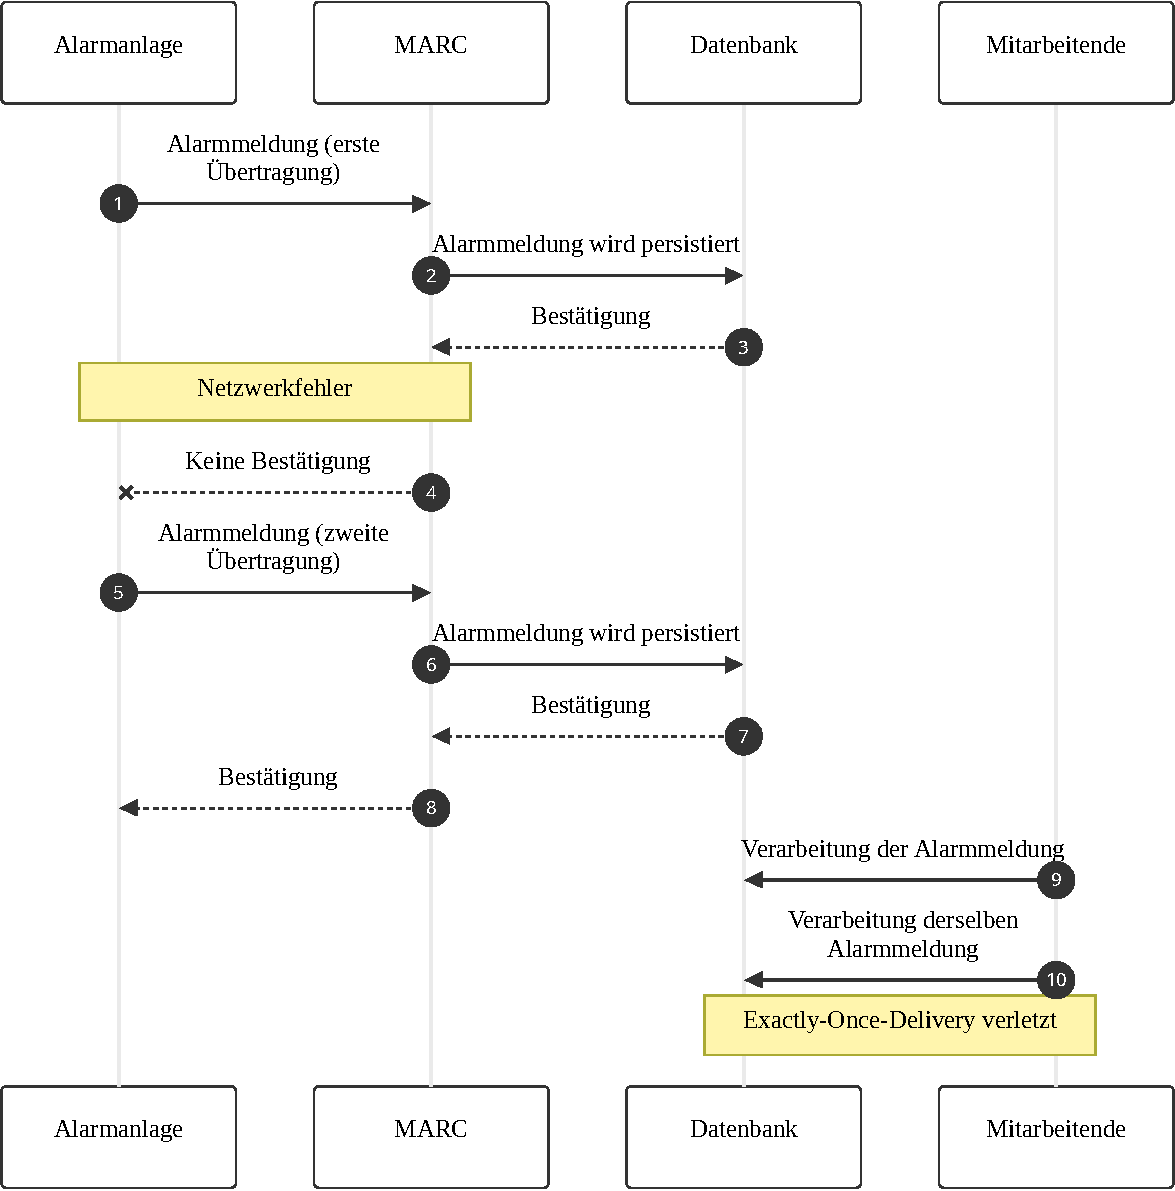
\includegraphics[width=0.653\textwidth]{./img/mermaid/marc_exactly_once_delivery_violation_sequence.pdf}
    \caption{Sequenzdiagramm eines beispielhaften Kommunikationsablaufs, der zu einer Verletzung der \textit{Exactly-Once-Delivery} im \acrshort{marc}-System führt.}
    \label{fig:exactly-once-diagram}
\end{figure}

Abbildung~\ref{fig:in-order-diagram} zeigt einen beispielhaften Kommunikationsablauf, der zu einer Verletzung der \textit{In-Order-Delivery} führt: Eine später erzeugte Alarmmeldung wird vor einer früheren Alarmmeldung verarbeitet, da variable Netzwerlatenzen die Reihenfolge verändern können.

\begin{figure}[H]
    \centering
    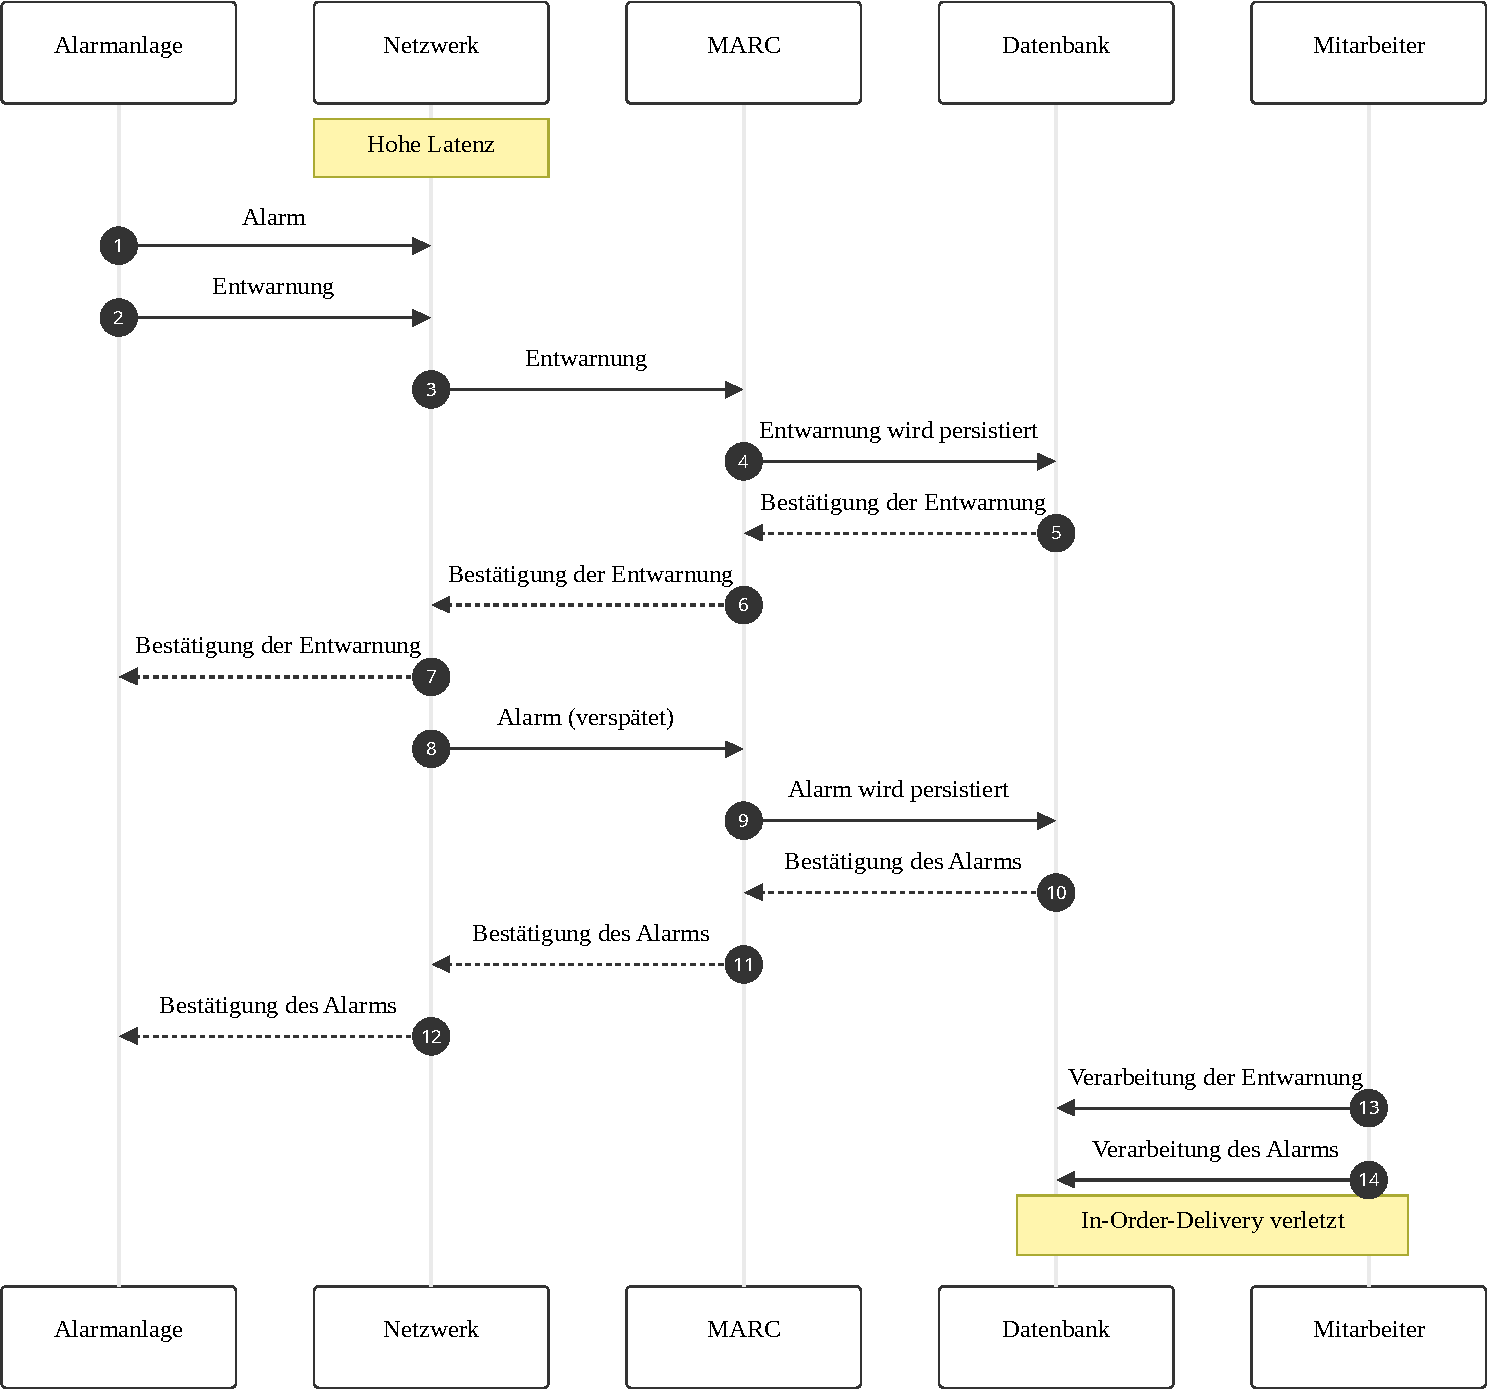
\includegraphics[width=0.826\textwidth]{./img/mermaid/marc_in_order_delivery_violation_sequence.pdf}
    \caption{Sequenzdiagramm eines beispielhaften Kommunikationsablaufs, der zu einer Verletzung der \textit{In-Order-Delivery} im \acrshort{marc}-System führt.}
    \label{fig:in-order-diagram}
\end{figure}

\section{Legacy Proxy System}
\label{sec:lps}

\subsection{Architektur}
\label{sub-sec:lps-architektur}

Nachdem in vorherigen Abschnitten das \gls{marc}-System beschrieben wurde, betrachtet dieser Abschnitt das in~\citep{liebig_2025_architectural_refactoring} vorgeschlagene \gls{lps}. Auf Basis der zuvor identifizierten Design Smells in Abschnitt~\ref{sec:design-smells} schlägt die Arbeit~\citep{liebig_2025_architectural_refactoring} ein Ar\-chi\-tek\-tur-Reengineering vor, um die Auswirkungen der identifizierten Design Smells zu mitigieren, ohne Modifikationen am Quellcode der Legacy-Services vorzunehmen. Der Kern dieses Ansatzes ist die transparente Integration des \gls{lps} zwischen den Services des \gls{marc}-Systems. Die Grundidee des \gls{lps} besteht in der Entkopplung der synchronen Verarbeitungskette zwischen den Services \gls{srv}~1 und \gls{srv}~2 durch eine \textit{Proxy-Broker-Proxy-Architektur}~\footnote{Eine Proxy-Broker-Proxy-Architektur bezeichnet ein Integrationsmuster, bei dem ein Message Broker von zwei Proxies gekapselt wird. Dies ermöglicht es, synchrone Kommunikationspfade transparent in eine asynchrone Kommunikationspfade zu überführen, ohne die bestehenden Schnittstellen der ursprünglichen Endpunkte anzupassen~\citep{hohpe2004enterprise}.}. Das \gls{lps} wird zwischen \gls{srv}~1 und \gls{srv}~2 positioniert und setzt sich aus drei Komponenten zusammen: dem \gls{lpone}, einem Message Broker und dem \gls{lptwo}. Abbildung~\ref{fig:lps-architektur} zeigt die transparente Integration von \gls{lps} in \gls{marc} zwischen \gls{srv}~1 und \gls{srv}~2. Die zuvor direkte synchrone Kopplung wird durch die Kette \textit{\gls{lpone} $\rightarrow$ Broker $\rightarrow$ \gls{lptwo}} ersetzt, sodass eingehende Alarmmeldungen zunächst entgegengenommen und im Broker gepuffert werden, bevor sie asynchron weiterverarbeitet werden. Die bestehende Legacy-Schnittstelle bleibt dabei nach außen unverändert.

\begin{figure}[htbp]
    \centering
    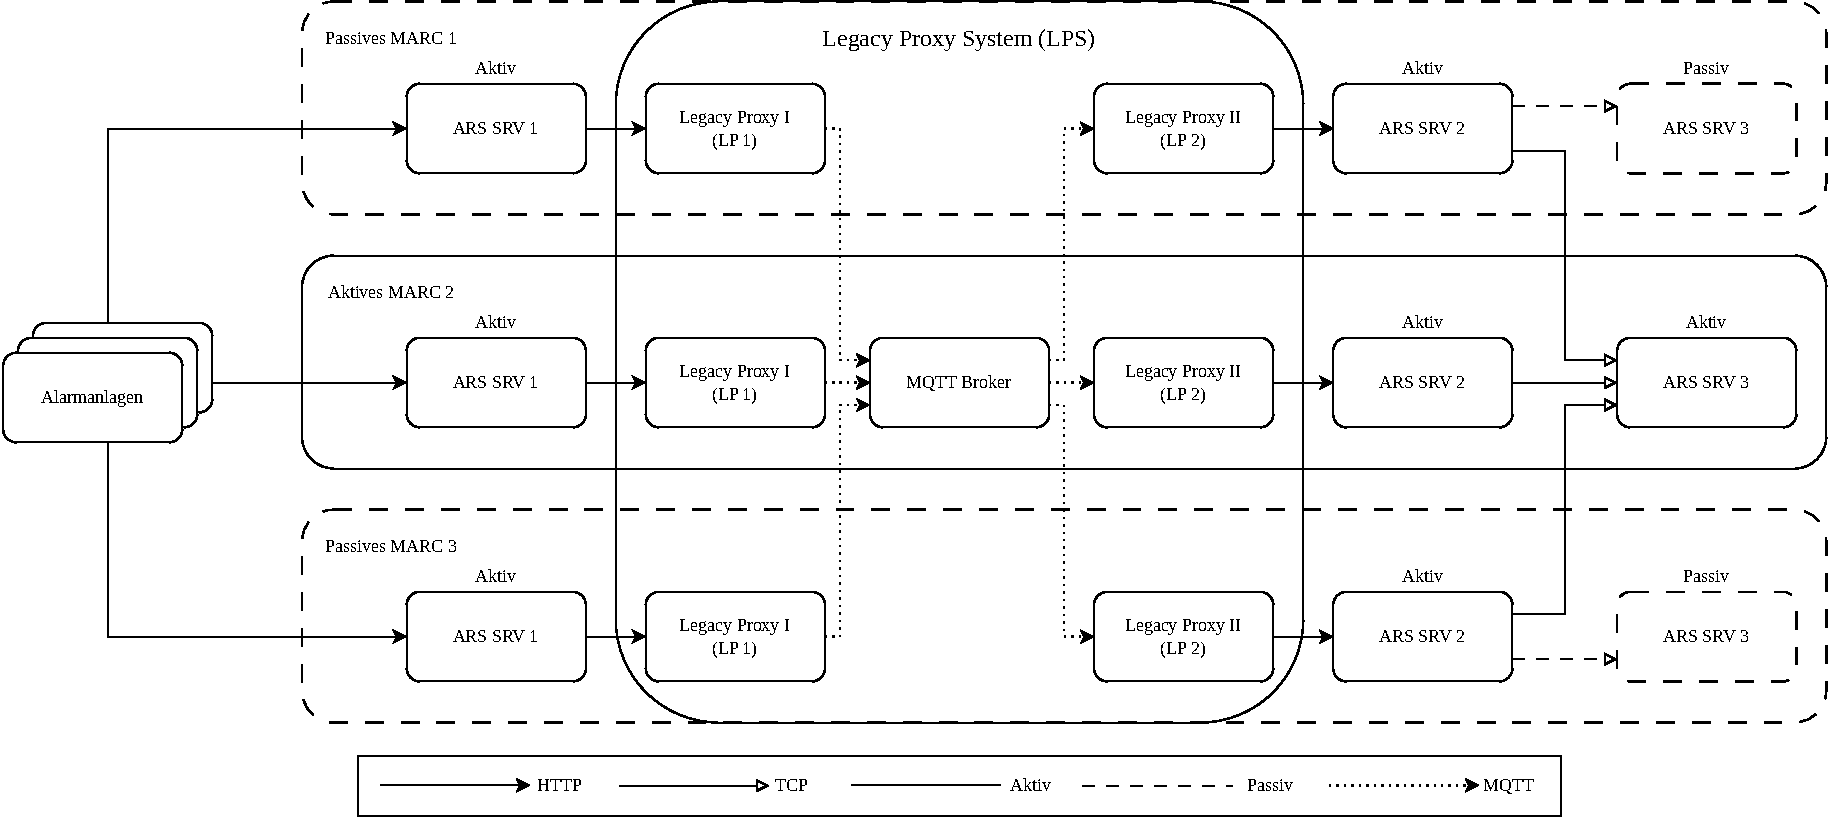
\includegraphics[width=\textwidth]{./img/drawio/lps.pdf}
    \caption{Gesamtarchitektur von \acrshort{marc} nach der Integration von \acrshort{lps}.}
    \label{fig:lps-architektur}
\end{figure}

In der Proof-of-Concept-Implementierung der Arbeit~\citep{liebig_2025_architectural_refactoring} wird das Protokoll \gls{mqtt}~v5 genutzt, um das \gls{lps} zu realisieren, wobei HiveMQ~\citep{hivemq_2025} als Broker zum Einsatz kommt. Im Normalbetrieb nimmt \gls{lpone} die Requests von \gls{srv}~1 entgegen und publiziert sie auf einem entsprechenden Topic, die im Folgendem als Main-Topic bezeichnet wird. Sobald der Broker den Eingang bestätigt, sendet \gls{lpone} unmittelbar eine Bestätigung an das vorgelagerte System zurück. Dadurch wird die synchrone Wartezeit der ursprünglichen Verarbeitungskette reduziert. Parallel dazu konsumiert \gls{lptwo} die Nachrichten aus dem Main-Topic und leitet sie asynchron an \gls{srv}~2 weiter. Abbildung~\ref{fig:lps-normalfluss} zeigt einen beispielhaften Verarbeitungsablauf einer Alarmmeldung innerhalb von \gls{lps} im Normalbetrieb. Unter Normalbetrieb wird die fehlerfreie Verarbeitung einer Alarmmeldung verstanden, bei der weder Netzwerkfehler noch negative Antworten der nachgelagerten Services (\gls{srv}~2, \gls{srv}~3) auftreten.

\begin{figure}[htbp]
    \centering
    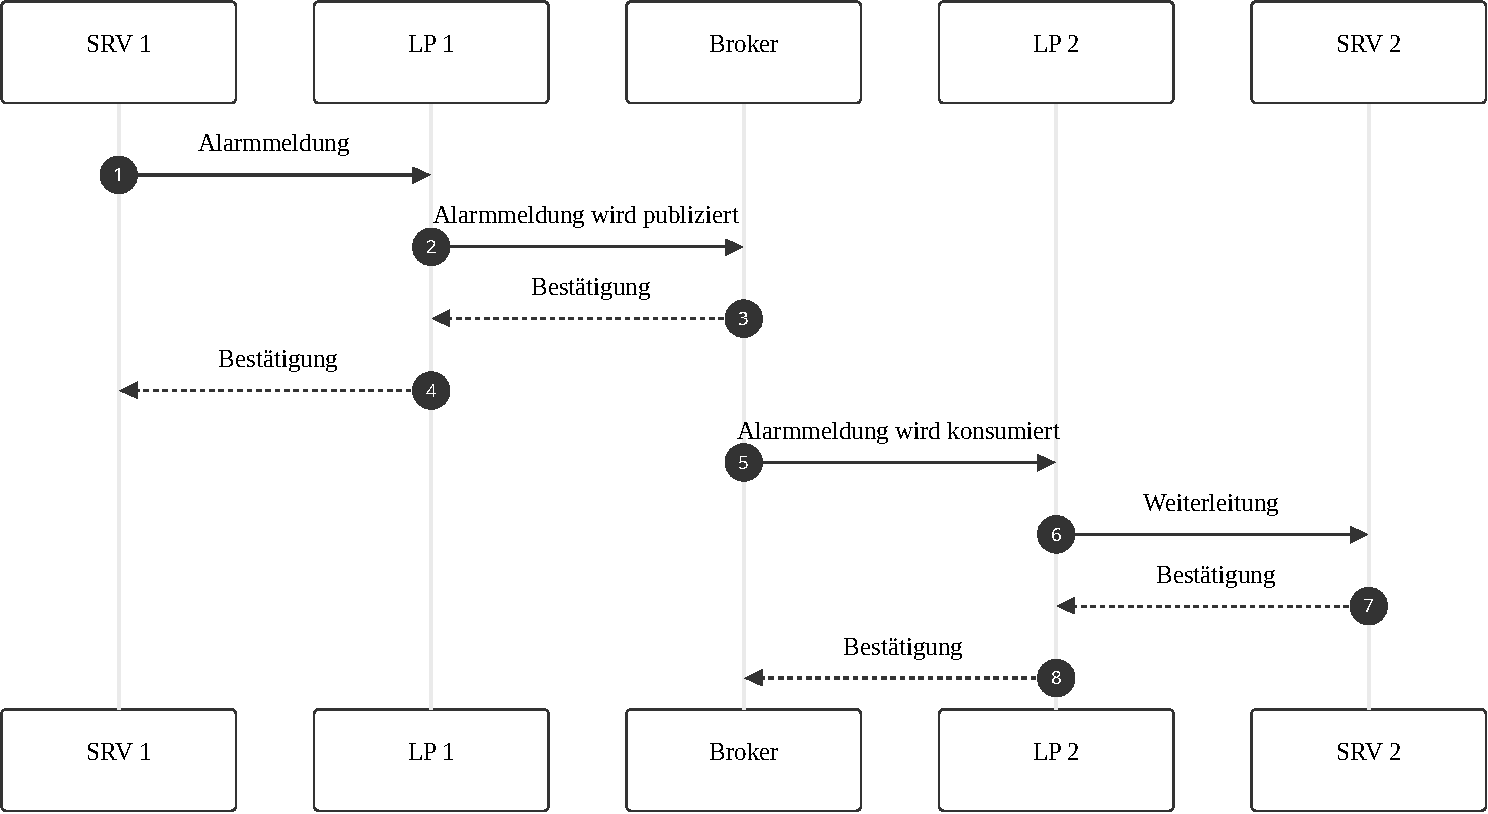
\includegraphics[width=0.826\textwidth]{./img/mermaid/lps_normal_sequence.pdf}
    \caption{Sequenzdiagramm eines beispielhaften Verarbeitungsablaufs einer Alarmmeldung innerhalb von \acrshort{lps} im Normalbetrieb.}
    \label{fig:lps-normalfluss}
\end{figure}

Um die strengen Delivery-Garantien des Legacy-Systems zu wahren, kombiniert \gls{lps} mehrere Mechanismen. Die Kommunikation zwischen \gls{lpone}, Broker und \gls{lptwo} erfolgt über \gls{mqtt} \gls{qos}~2, was eine \textit{Exactly-Once-Delivery} auf diesem Teilpfad garantiert. Um die \textit{In-Order-Delivery} der Alarmmeldungen zu gewährleisten, werden die \gls{lptwo}-Instanzen so konfiguriert, dass Nachrichten innerhalb derselben Instanz anhand von \texttt{max\_\allowbreak inflight\_\allowbreak messages = 1} sequentiell verarbeitet werden. Für Fehlerfälle wie Netzwerkfehler oder negative Antworten der nachgelagerten Services, die hinter \gls{lptwo} auftreten, wird ein \textit{Retry}-Mechanismus~\footnote{Retry bezeichnet das erneute Zustellen einer zuvor fehlgeschlagenen Nachricht.} eingeführt. Bei fehlgeschlagener Über\-tra\-gung einer Alarmmeldung an die nachgelagerten Services, wird diese Alarmmeldung auf ein separates Topic, die im Folgendem als Retry-Topic bezeichnet wird, publiziert. Der Retry-Mechanismus wird durch eine Broker-Erweiterung (Plugin) umgesetzt, die Nachrichten aus dem Retry-Topic strikt priorisiert. Sobald sich Nachrichten im Retry-Topic befinden, wird die Auslieferung regulärer Nachrichten aus dem Main-Topic temporär pausiert. Erst nach der erfolgreichen Verarbeitung der Retry-Nachrichten wird der reguläre Nachrichtenfluss fortgesetzt. Dies verhindert, dass neuere Alarmmeldungen eine ältere, zuvor fehlgeschlagene Alarmmeldung überholen. Der Ablauf dieses Mechanismus gestaltet sich wie folgt:

\begin{enumerate}
    \item \gls{lpone} publiziert eine Alarmmeldung in das Main-Topic.
    \item \gls{lptwo} konsumiert die Alarmmeldung aus dem Main-Topic und versucht sie an \gls{srv}~2 weiterzuleiten.
    \item Im Fehlerfall wird die Alarmmeldung in das Retry-Topic publiziert.
    \item Das Broker-Plugin pausiert die Auslieferung von reguläreren Nachrichten aus dem Main-Topic und priorisiert die Auslieferung der Nachrichten aus dem Retry-Topic.
    \item Nach erfolgreicher Verarbeitung aller Nachrichten im Retry-Topic wird die Auslieferung von reguläreren Nachrichten fortgesetzt.
\end{enumerate}

Abbildung~\ref{fig:lps-retry-priorisierung} zeigt einen beispielhaften Verarbeitungsablauf einer Alarmmeldung innerhalb von \gls{lps} im Fehlerfall.

\begin{figure}[htbp]
    \centering
    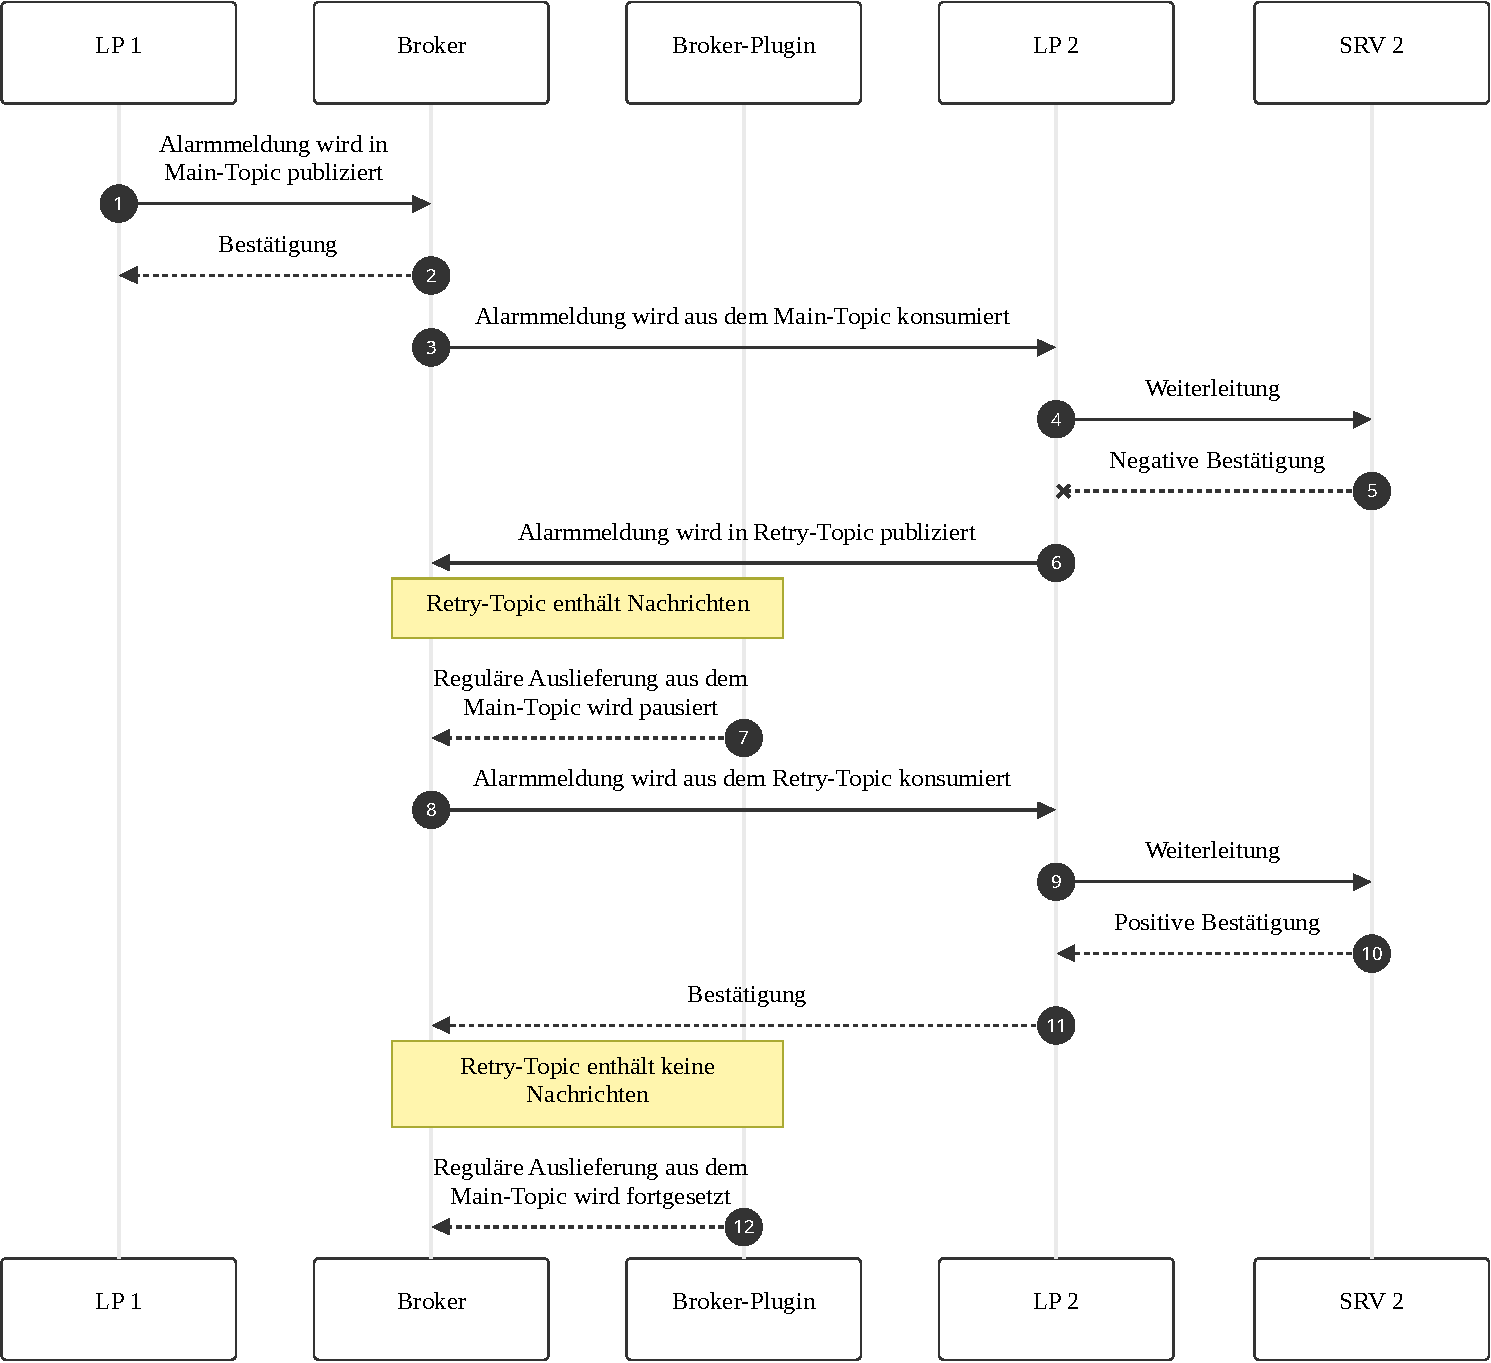
\includegraphics[width=0.828\textwidth]{./img/mermaid/lps_retry_prio_sequence.pdf}
    \caption{Sequenzdiagramm eines beispielhaften Verarbeitungsablaufs einer Alarmmeldung innerhalb von \acrshort{lps} im Fehlerfall.}
    \label{fig:lps-retry-priorisierung}
\end{figure}

\subsection{Auswirkungen auf die Design Smells}
\label{sub-sec:lps-auswirkungen}

Durch die Integration von \gls{lps} werden die Auswirkungen der zuvor identifizierten Design Smells in Abschnitt~\ref{sec:design-smells} mitigiert:

\begin{itemize}
    \item \textbf{Smell~1}: \textit{Synchrone Request-Response-Ketten}. Die direkte synchrone Kopplung zwischen \gls{srv}~1 und \gls{srv}~2 wird aufgrund der asynchronen Verarbeitung der Alarmmeldungen durch die \textit{Proxy-Broker-Proxy-Archi\-tek\-tur} aufgebrochen. \gls{lpone} bestätigt den Eingang einer Alarmmeldung an die vorgelagerten Services direkt nach dem Publizieren der Alarmmeldung an das Broker. Dadurch wird die Latenzakkumulation entlang der Verarbeitungskette reduziert.

    \item \textbf{Smell~2}: \textit{Heterogene Redundanzmodi}. die \textit{Proxy-Broker-Proxy-Archi\-tek\-tur} und der Einsatz mehrerer \gls{lptwo}-Instanzen machen das System widerstandsfähiger gegenüber Ausfällen oder Netzwerkverbindungen.

          % TODO: TF is this?
    \item \textbf{Smell~3}: \textit{Manuelles Ausfall-Management}. Zwar bleibt die Notwendigkeit manueller Eingriffe bei schwerwiegenden Ausfällen formal bestehen, jedoch werden die unmittelbaren negativen Auswirkungen auf die Antwortzeiten vorgelagerter Systeme reduziert, da eingehende Alarmmeldungen sicher im Broker zwischengespeichert werden.

    \item \textbf{Smell~4 \& Smell~5}: \textit{Exactly-Once-Delivery} \& \textit{In-Order-Delivery} werden über \gls{qos}~2 und das Retry-Mechanismus adressiert.
\end{itemize}

Zur Validierung des Ansatzes wurden abschließend Experimente durchge\-führt, bei denen simulierte Alarmanlagen Alarmmeldungen an das senden. Der Fokus der Experimente lag auf der Reduktion der Antwortzeiten sowie der Einhaltung der \textit{Exactly-Once-Delivery}. Die Experimente belegten, dass die Antwortzeiten des Systems nach dem Integrieren von \gls{lps} sowohl im Normalbetrieb als auch in Fehlerszenarien verbessert wurden und das System die Vorgaben der europäischen Norm EN 50136~\citep{din_en_50136-12012-08_alarm_2012} erfüllt. Die Garantie der \textit{Exactly-Once-Delivery} und \textit{In-Order-Delivery} konnten laut den Experimenten ebenso gewahrt werden.

\subsection{Limitationen der Experimente}
\label{sub-sec:lps-limitationen-experimente}

Nach dem Betrachten der durchgeführten Experimente und der Interpretation der Ergebnisse ergeben sich potentiale Verletzungen der Delivery-Garantien. Laut dem Paper wird die Einhaltung von \textit{Exactly-Once-Delivery} bestätigt, in dem die Anzahl gesendeter Alarmmeldungen der simulierten Alarmanlagen gleich der Anzahl angekommener Alarmmeldung. Jedoch ist der Vergleich der Anzahl nicht ausreichend, um die \textit{Exactly-Once-Delivery} zu bestätigen. Eine beispielhafte Sequenz von Alarmmeldungen, die zur Verletzung von \textit{Exactly-Once-Delivery} sieht folgendermaßen aus: Die Alarmanlage \texttt{A} sendet die Alarmmeldungen \texttt{\#1} und \texttt{\#2}. Alarmmeldung~\texttt{\#1} geht im Netz verloren, während Alarmmeldung~\texttt{\#2} dupliziert ankommt. Die Anzahl gesendeter Alarmmeldungen ist gleich der Anzahl angekommener Alarmmeldungen, jedoch ist Alarmmeldung~\texttt{\#2} mehrfach angekommen. Außerdem wird die globale \textit{In-Order-Delivery} in den Experimenten nicht betrachtet. Innerhalb der \gls{lptwo}-Instanzen werden Alarmmeldungen anhand von (\texttt{max\_inflight\_messages = 1}) sequentiell bearbeitet. Dadurch garantiert \gls{lptwo} \textit{In-Order-Delivery} innerhalb einer Instanz, jedoch keine globale \textit{In-Order-Delivery}. Aufgrund der \textit{shared subscriptions} ist es möglich, dass zwei \gls{lptwo}-Instanzen Alarmmeldungen gleichzeitig bearbeiten. Das kann bei variablen Verarbeitungszeiten der Alarmmeldungen in den nachgelagerten Services dazu führen, dass Alarmmeldungen in der falschen Reihenfolge in der Datenbank gespeichert werden. Im nächsten Abschnitt werden Experimente durchgeführt, bei denen die Verletzung der Delivery-Garantien gezielt provoziert wird.

\subsection{Experimente}
\label{sub-sec:lps-experimente}

Die in diesem Abschnitt durchgeführten Experimente umfassen zwei Simulationen des Legacy-Systems nach dem Integrieren von \gls{lps}. Bei den Simulationen werden Alarmanlagen simuliert, die Alarmmeldungen periodisch an das System senden. Die gesendeten Alarmmeldungen bestehen hauptsächlich aus zwei Feldern: \texttt{device\_id} und \texttt{triggertime}. \texttt{device\_id} ist der Identifikator einer Alarmanlage und \texttt{triggertime} ist der Identifikator einer Alarmmeldung. Es ist garantiert, dass die \texttt{triggertime} der gesendeten Alarmmeldungen monoton steigend ist. Außerdem sind die simulierten Alarmanlagen so eingestellt, dass sie das Übertragen von Alarmmeldungen erneut versuchen, falls Fehler beim Übertragen auftreten. Wiederholte Alarmmeldungen besitzen die gleiche \texttt{triggertime} wie die ursprünglich fehlgeschlagene Alarmmeldung. Die nachgelagerten Services von \gls{lps}, nämlich \gls{srv}~2 und \gls{srv}~3, werden durch einen Service simuliert, dessen Aufgabe es ist, Alarmmeldungen von \gls{lps} bzw.~\gls{lptwo} zu empfangen und zu speichern. Die gespeicherten Alarmmeldungen werden abschließend auf \textit{Exactly-Once-Delivery} und \textit{In-Order-Delivery} geprüft. Zum Ausführen der Experimente werden vier Hilfsservices eingeführt:

\begin{itemize}
    \item \textbf{Alarmanlagen-Simulator:} Der Alarmanlagen-Simulator bildet externe Alarmanlagen nach und erzeugt periodisch Alarmmeldungen, die an das System gesendet werden. Die gesamte Anzahl simulierter Alarmanlagen ($N_{\text{device}}$) sowie die Anzahl gesendeter Alarmmeldungen pro Alarmanlage ($N_{\text{alarm}}$) sind einstellbar. Außerdem sind die minimale ($I_{\text{min,alarm}}$) und die maximale Wartezeit ($I_{\text{max,alarm}}$) zwischen zwei gesendeten Alarmmeldungen einer Alarmanlage einstellbar. Die tatsächliche Wartezeit wird vor jeder Alarmmeldung zufällig zwischen $I_{\text{min,alarm}}$ und $I_{\text{max,alarm}}$ bestimmt. Gilt hingegen $I_{\text{min,alarm}} = I_{\text{max,alarm}}$, ergibt sich ein festes Sendeintervall ($I_{\text{alarm}}$), sodass die Alarmmeldungen einer Alarmanlage in exakt gleichen zeitlichen Abständen gesendet werden. Erfolgreich gesendete Alarmmeldungen werden abschließend in einer Datei gespeichert (\texttt{device-results.\allowbreak json}).

    \item \textbf{\gls{tcp}-Proxy:} Der \gls{tcp}-Proxy dient zur gezielten Simulation von Netzwerkfehlern zwischen Komponenten des simulierten Systems. Der \gls{tcp}-Proxy lehnt Verbindungen mit einer einstellbaren Fehlerrate ($E_{\text{tcp}}$) zu\-fäl\-lig ab und leitet akzeptierte Verbindungen an die Zieladresse weiter. Die minimale ($T_{\text{min,tcp}}$) und die maximale Dauer ($T_{\text{max,tcp}}$) einer akzeptierten Verbindung sind einstellbar; die tatsächliche Dauer wird für jede Verbindung zufällig zwischen $T_{\text{min,tcp}}$ und $T_{\text{max,tcp}}$ bestimmt. Analog zum Alarmanlagen-Simulator ergibt sich bei $T_{\text{min,tcp}} = T_{\text{max,tcp}}$ eine feste Verbindungsdauer ($T_{\text{tcp}}$), sodass jede Verbindung nach exakt derselben Dauer getrennt wird. Nach Ablauf dieser Dauer wird die Verbindung getrennt, was zu einem Netzwerkfehler zwischen den beteiligten Komponenten führt. Abschließend werden die Zeitstempel, an denen eine Verbindung getrennt wurde, in einer Datei gespeichert (\texttt{tcp-proxy-results.\allowbreak json}).

    \item \textbf{Server-Simulator:} Der Server-Simulator simuliert die nachgelagerten Services \gls{srv}~2 und \gls{srv}~3 und stellt damit den Endpunkt der experimentellen Verarbeitungskette dar. Der Server-Simulator empfängt Alarmmeldungen von \gls{lps} bzw.~\gls{lptwo} und antwortet mit einer einstellbaren Fehlerrate ($E_{\text{server}}$) zufällig mit einer positiven oder negativen Bestätigung. Dadurch bildet der Server-Simulator echte Verarbeitungsfehler in den nachgelagerten Services \gls{srv}~2 und \gls{srv}~3 nach. Außerdem sind die minimale ($T_{\text{min,server}}$) und die maximale Verarbeitungszeit ($T_{\text{max,server}}$) einer Alarmmeldung einstellbar; die tatsächliche Verarbeitungszeit wird für jede Alarmmeldung zufällig zwischen $T_{\text{min,server}}$ und $T_{\text{max,server}}$ bestimmt. Analog zum Alarmanlagen-Simulator ergibt sich bei $T_{\text{min,server}} = T_{\text{max,server}}$ eine feste Verarbeitungszeit ($T_{\text{server}}$), sodass jede Alarmmeldung exakt gleich lange verarbeitet wird. Dadurch simuliert der Server beliebige Verarbeitungszeiten der nachgelagerten Services \gls{srv}~2 und \gls{srv}~3 sowie variable Über\-tra\-gungs\-laten\-zen im Netz. Der Server-Simulator ist außerdem mit einer einstellbaren Idle-Zeit ($T_{\text{idle}}$) konfigurierbar. Die Idle-Zeit dient dazu, den Server-Simulator zu terminieren und somit die Simulation zu beenden, nachdem eine bestimmte Zeit lang keine Alarmmeldungen mehr empfangen wurden. Abschließend werden erfolgreich verarbeitete Alarmmeldungen in einer Datei gespeichert (\texttt{server-results.\allowbreak json}).

    \item \textbf{Validator:} Der Validator wird immer nach Abschluss einer Simulation ausgeführt und vergleicht die vom Alarmanlagen-Simulator gesendeten Alarmmeldungen mit den beim Server-Simulator angekommenen Alarmmeldungen. Konkret werden die Vollständigkeit der Zustellung der Alarmmeldungen sowie die Einhaltung der \textit{In-Order-Delivery} und \textit{Exactly-Once-Delivery} validiert. Die Vollständigkeit der Alarmmeldungen wird validiert, indem geprüft wird, dass jede gesendete Alarmmeldung aus \texttt{device-\allowbreak results} mindestens einmal in \texttt{server-\allowbreak results} vorkommt. Die \textit{Exactly-Once-Delivery} wird dadurch validiert, dass jede gesendete Alarmmeldung aus \texttt{device-\allowbreak results} höchstens einmal in \texttt{server-\allowbreak results} vorkommt. Die \textit{In-Order-Delivery} wird pro Alarmanlage validiert, indem zunächst mehrfach angekommene Alarmmeldungen entfernt werden und danach geprüft wird, ob alle Alarmmeldungen jeder einzelnen Alarmanlage anhand des Felds \texttt{triggertime} monoton steigend sind. Jede Verletzung der Monotonie einer Alarmanlage wird als \textit{Außer Reihenfolge} klassifiziert. Zur Veranschaulichung der Validierung von \textit{In-Order-Delivery} wird die folgende Sequenz empfangener Alarmmeldungen betrachtet:

          \begin{table}[H]
              \centering
              \begin{tabular}{|l|l|l|}
                  \hline
                  \textbf{Index} & \textbf{device\_id} & \textbf{triggertime} \\
                  \hline
                  \#1            & 1                   & 0                    \\
                  \#2            & 1                   & 2                    \\
                  \#3            & 1                   & 3                    \\
                  \#4            & 1                   & 1                    \\
                  \#5            & 1                   & 4                    \\
                  \hline
              \end{tabular}
              \caption{Beispielhafte Sequenz empfangener Alarmmeldungen zur Veranschaulichung der In-Order-Delivery Validierung.}
              \label{tab:in-order-delivery-seq-beispiel}
          \end{table}

          Alarmmeldung~\#4 ist in der falschen Reihenfolge angekommen, da ihre \texttt{triggertime} kleiner als die \texttt{triggertime} der vorherigen Alarmmeldung~\#3 ist. Alarmmeldung~\#5 ist laut der Validierung hingegen in der richtigen Reihenfolge angekommen, da ihre \texttt{triggertime} größer als die der vorherigen Alarmmeldung~\#4 ist. Diese Validierung dient nicht als quantitative Metrik zum Zählen von \textit{Außer Reihenfolge} angekommenen Alarmmeldungen, sondern als qualitative Metrik, die die Verletzung der \textit{In-Order-Delivery} aufzeigt. Die genaue Anzahl der \textit{Außer Reihenfolge} angekommenen Alarmmeldungen kann je nach verwendetem Algorithmus variieren. Beispielsweise kann ein Algorithmus die Alarmmeldungen~\#2 und \#3 als \textit{Außer Reihenfolge} klassifizieren, da sie vor der Alarmmeldung~\#4 mit einer kleineren \texttt{triggertime} angekommen sind.
\end{itemize}

Für die Durchführung der Experimente wird die originale Implementierung von \gls{lps} aus dem offiziellen GitHub-Repository~\citep{legacy_proxy_pattern_repo} herangezogen. Die Implementierung umfasst die Komponenten \textit{\gls{lpone}}, \textit{\gls{lptwo}} und das eigens entwickelte Broker-Plugin für den Retry-Mechanismus sowie zwei Hilfsservices \textit{\gls{srv}~1 PROXY} und \textit{\gls{srv}~2 PROXY}, die die Kommunikation zwischen \gls{lpone} und \gls{srv}~1 sowie zwischen \gls{lptwo} und \gls{srv}~2 ermöglichen. Nach dem Zusammenstellen der beteiligten Komponenten ergibt sich die in Abbildung~\ref{fig:exp-setup} dargestellte Architektur der Experimente.

\begin{figure}[H]
    \centering
    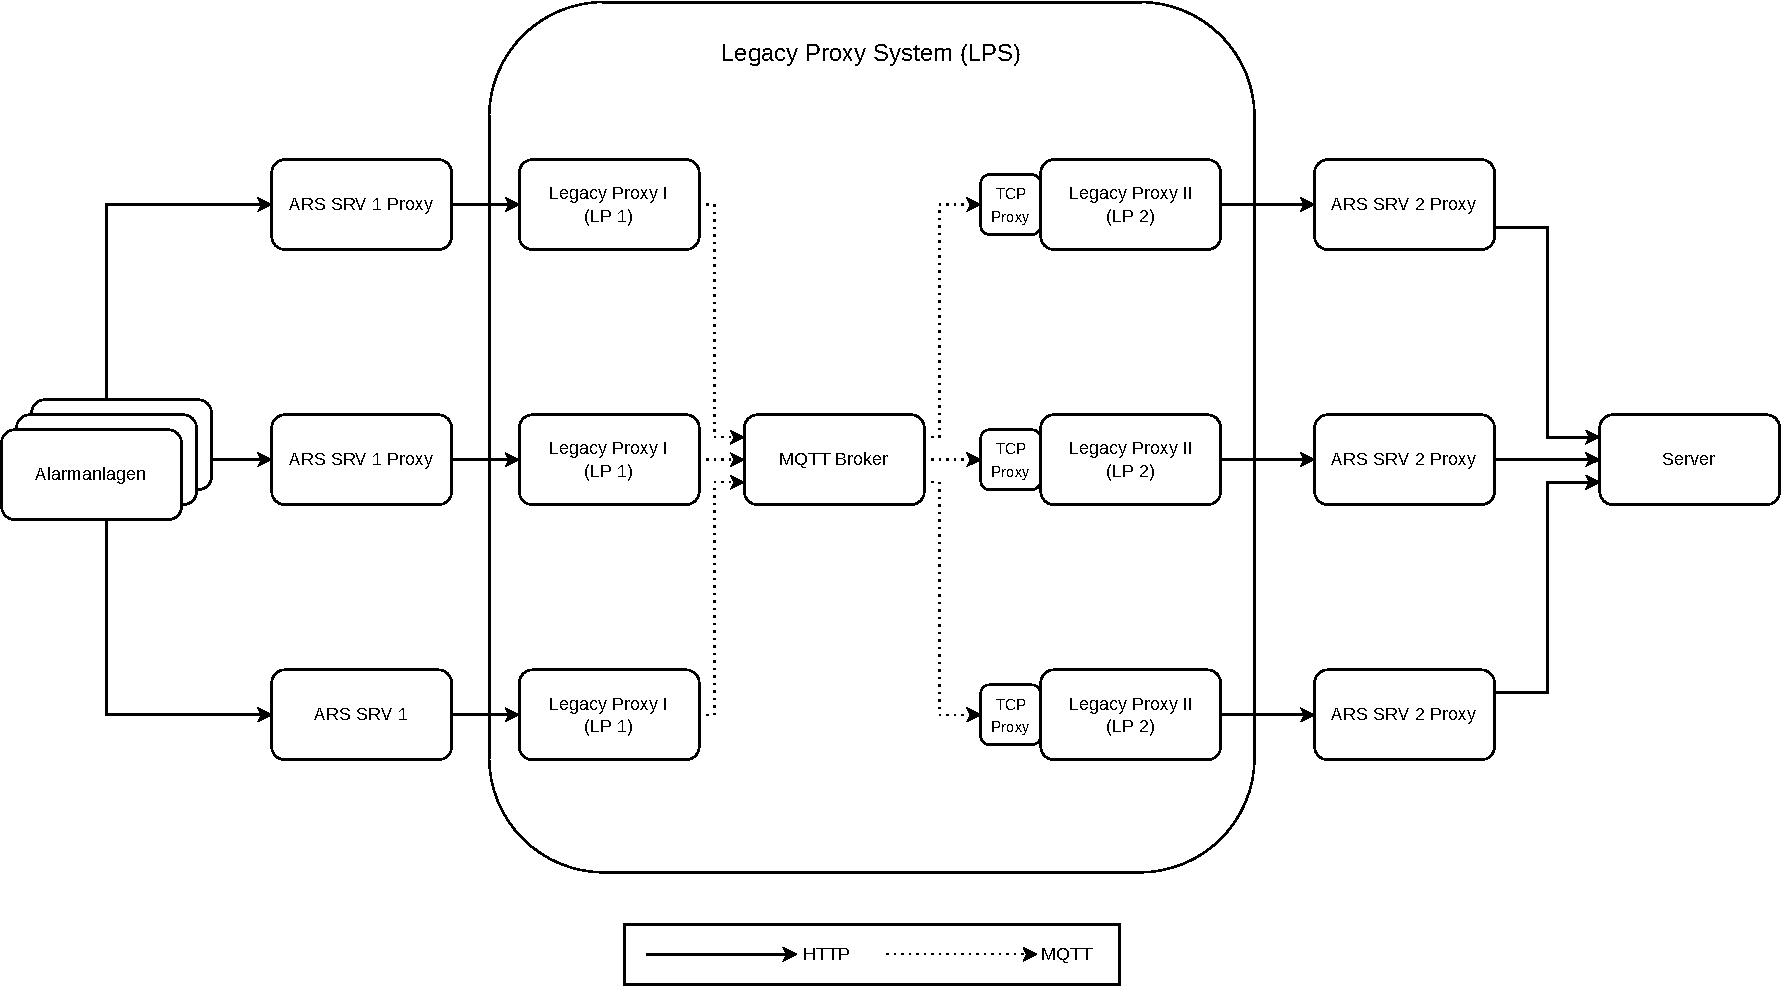
\includegraphics[width=\textwidth]{./img/drawio/exp_lps.pdf}
    \caption{Architektur der Experimente von \acrshort{lps} und Kommunikationspfade der beteiligten Komponenten.}
    \label{fig:exp-setup}
\end{figure}

Abbildung~\ref{fig:exp-setup} veranschaulicht die Architektur der durchgeführten Experimente sowie die Interaktionen der einzelnen Komponenten. Der \textit{Alarmanlagen-Simulator} generiert periodisch Alarmmeldungen und sendet sie per \gls{http} an den \textit{\gls{srv}~1 PROXY}. Dieser nimmt die Alarmmeldungen entgegen und leitet sie an \gls{lpone} weiter. \gls{lpone} publiziert die empfangenen Alarmmeldungen an den Broker. Sobald der Broker den Eingang bestätigt, sendet \gls{lpone} eine positive Bestätigung zurück, die über den \textit{\gls{srv}~1 PROXY} beim \textit{Alarmanlagen-Simulator} ankommt und die erfolgreiche Übertragung signalisiert. Die \gls{lptwo}-Instanzen verbinden sich über die \textit{\gls{tcp}-Proxies} mit dem Broker, konsumieren die Alarmmeldungen aus dem Broker und leiten sie über den \textit{\gls{srv}~2 PROXY} weiter. Dieser übergibt die Alarmmeldungen abschließend an den \textit{Server-Simulator}, der die Verarbeitung und Speicherung der Alarmmeldungen übernimmt und somit die Rolle der ursprünglichen Services \gls{srv}~2 und \gls{srv}~3 von \textit{\gls{marc}} einnimmt. Die \textit{\gls{tcp}-Proxies} werden gezielt zwischen den \gls{lptwo}-Instanzen und dem Broker positioniert, um Netzwerkfehler auf diesem Pfad zu provozieren, die zu einer Verletzung der \textit{Exactly-Once-Delivery} führen können, wie in Abschnitt~\ref{sub-sub:alp-verletzung-eod} beschrieben wird. Alle übrigen Kommunikationspfade werden als fehlerfrei angenommen, da sie für die Verletzung der Delivery-Garantien in den Experimenten keine Rolle spielen.

\subsubsection{Reproduzierbarkeit und Anzahl der Durchläufe}
\label{sub-sub:lps-methodik}

Die Experimente sind stochastisch, da Verarbeitungszeiten, Verbindungsdauern und Fehler zufällig erzeugt werden. Damit die Experimente reproduzierbar sind, werden alle Zufallswerte von einem Pseudozufallszahlengenerator erzeugt, der mit einem einstellbaren Seed $S$ initialisiert wird. Der Seed wird allen Hilfsservices übergeben, die Zufallswerte erzeugen, also dem \textit{Alarmanlagen-Simulator}, dem \textit{\gls{tcp}-Proxy} und dem \textit{Server-Simulator}. Bei gleichem Seed erzeugen diese Services in jedem Durchlauf dieselbe Folge von Zufallswerten. Der Seed legt jedoch nicht das gesamte zeitliche Verhalten des Systems fest: Das Scheduling durch das \gls{os}, der Verbindungsaufbau sowie die Verarbeitungszeiten des Brokers und der \gls{lps}-Komponenten werden nicht durch den Seed gesteuert. Daher können sich Durchläufe mit demselben Seed in ihren Ergebnissen unterscheiden, beispielsweise in der Anzahl entstandener Duplikate. Aus dem Ergebnis eines einzelnen Durchlaufs lässt sich somit keine belastbare Aussage ableiten. Aus diesem Grund wird jedes Experiment mit demselben Seed mehrfach wiederholt. Die Anzahl der benötigten Wiederholungen $n$ wird nach dem \textit{Success-Run-Theorem}~\citep{joshi2023, kececioglu1992} bestimmt:

\begin{equation}
    n = \frac{\ln(1 - C)}{\ln(R)}
    \label{eq:success-run}
\end{equation}

Dabei ist $R$ die Zuverlässigkeit (\textit{Reliability}): Die minimale Wahrscheinlichkeit, mit der ein einzelner Durchlauf ein zuvor festgelegtes Erfolgskriterium erfüllt. $C$ ist die Konfidenz (\textit{Confidence}), mit der diese Aussage getroffen werden soll. In dieser Masterarbeit werden $R = 95\,\%$ und $C = 95\,\%$ verwendet. Diese Kombination ist in der Zuverlässigkeitsprüfung und Prozessvalidierung gängig~\citep{qualitymag, schenkelberg2024}. Daraus ergibt sich:

\begin{equation}
    n = \frac{\ln(1 - 0{,}95)}{\ln(0{,}95)} \approx 58{,}4 \;\rightarrow\; n = 59
    \label{eq:success-run-n}
\end{equation}

Jedes Experiment wird somit 59-mal wiederholt. Erfüllen alle 59 Durchläufe das Erfolgskriterium, kann mit einer Konfidenz von 95\,\% behauptet werden, dass ein einzelner Durchlauf das Erfolgskriterium mit einer Wahrscheinlichkeit von mindestens 95\,\% erfüllt. Verfehlt hingegen mindestens ein Durchlauf das Erfolgskriterium, kann diese Aussage nicht getroffen werden. In den folgenden Experimenten zu \gls{lps} gilt ein Durchlauf als erfolgreich, wenn die jeweils untersuchte Delivery-Garantie verletzt wird. Dadurch wird gezeigt, dass die Verletzung nicht nur zufällig in einem einzelnen Durchlauf auftritt, sondern sich mit dem gewählten Seed reproduzierbar provozieren lässt. Der Seed wird für jedes Experiment wie folgt bestimmt: Das Experiment wird mit verschiedenen Seeds ausgeführt, bis ein Seed gefunden wird, mit dem die untersuchte Verletzung konsistent auftritt. Anschließend wird das Experiment mit diesem Seed 59-mal wiederholt. Die gezielte Auswahl des Seeds ist zulässig, da die Experimente nicht die Häufigkeit einer Verletzung unter beliebigen Bedingungen messen, sondern zeigen sollen, dass \gls{lps} die Delivery-Garantien unter bestimmten Fehlerbedingungen verletzt. Der Seed legt diese Fehlerbedingungen fest und macht sie reproduzierbar.

\subsubsection{Verletzung der Exactly-Once-Delivery}
\label{sub-sub:alp-verletzung-eod}

In diesem Abschnitt wird ein Experiment durchgeführt, das gezielt eine Verletzung der \textit{Exactly-Once-Delivery} Garantie in \gls{lps} provoziert. Konkret wird die \gls{tcp}-Verbindung zwischen \gls{lptwo} und dem Broker während der Verarbeitung einer Alarmmeldung unterbrochen. Dadurch wird die gleiche Alarmmeldung mehrfach verarbeitet, was zu einer Verletzung der \textit{Exactly-Once-Delivery} führt. Dafür werden die Parameter in Tabelle~\ref{tab:exp-lps-eod-config} ausgewählt. Die quantitativen Parameter $N_{\text{lp~1}}$, $N_{\text{lp~2}}$, $N_{\text{device}}$ und $N_{\text{alarm}}$ werden so gewählt, dass die minimale Anzahl generierter Alarmmeldungen sowie beteiligter Komponenten verwendet wird, mit der eine Verletzung der \textit{Exactly-Once-Delivery} auftreten kann. Die zeitlichen Parameter $T_{\text{max,server}}$ und $T_{\text{max,tcp}}$ werden so gewählt, dass ein Netzwerkfehler zwischen \gls{lptwo} und dem Broker provoziert wird, während \gls{lptwo} eine Alarmmeldung verarbeitet und auf eine Antwort von den nachgelagerten Services wartet. Dabei stellen $T_{\text{max,server}}$ und $T_{\text{max,tcp}}$ lediglich Obergrenzen dar. Die tatsächliche Verarbeitungszeit sowie die tatsächliche Verbindungsdauer werden jeweils zufällig zwischen dem entsprechenden Minimalwert $T_{\text{min,server}}$ bzw.~$T_{\text{min,tcp}}$ (jeweils 0\,s) und dem entsprechenden Maximalwert bestimmt. Wären die Werte fest, also $T_{\text{min,server}} = T_{\text{max,server}}$ und $T_{\text{min,tcp}} = T_{\text{max,tcp}}$ (z.\,B.~genau 5\,s Verarbeitung und 4\,s Verbindung), würde jede Verbindung vor Abschluss der Verarbeitung getrennt, sodass \gls{lptwo} die Alarmmeldung nie bestätigen könnte. Der Broker würde sie daher endlos erneut zustellen und die Simulation würde nicht terminieren. Durch die Zufälligkeit wird die Verarbeitung hingegen irgendwann innerhalb der Verbindungsdauer abgeschlossen, die Alarmmeldung bestätigt und die Simulation nach $T_{\text{idle}}$ beendet. Als Seed wird $S = 3$ verwendet. Dieses Experiment wurde mit \textit{HiveMQ CE} in Version \textit{2025.5} durchgeführt.

\begin{table}[H]
    \centering
    \caption{Konfiguration des Experiments zur Verletzung der Exactly-Once-Delivery in \acrshort{lps}.}
    \label{tab:exp-lps-eod-config}
    \begin{tabular}{|l|l|l|}
        \hline
        \textbf{Parameter}      & \textbf{Beschreibung}                        & \textbf{Wert} \\
        \hline
        $N_{\text{lp~1}}$       & Anzahl \gls{lpone}-Instanzen                 & 1             \\
        $N_{\text{lp~2}}$       & Anzahl \gls{lptwo}-Instanzen                 & 1             \\
        $N_{\text{device}}$     & Anzahl Alarmanlagen                          & 1             \\
        $N_{\text{alarm}}$      & Anzahl Alarmmeldungen pro Alarmanlage        & 1             \\
        $T_{\text{min,server}}$ & Minimale Server-Verarbeitungszeit            & 0\,s          \\
        $T_{\text{max,server}}$ & Maximale Server-Verarbeitungszeit            & 5\,s          \\
        $E_{\text{server}}$     & Serverfehlerrate                             & 0{,}0\,\%     \\
        $T_{\text{idle}}$       & Server-Idle-Zeit                             & 5\,s          \\
        $E_{\text{tcp}}$        & \gls{tcp}-Fehlerrate                         & 0{,}0\,\%     \\
        $T_{\text{min,tcp}}$    & Minimale Verbindungsdauer im \gls{tcp}-Proxy & 0\,s          \\
        $T_{\text{max,tcp}}$    & Maximale Verbindungsdauer im \gls{tcp}-Proxy & 4\,s          \\
        $S$                     & Seed des Pseudozufallszahlengenerators       & 3             \\
        \hline
    \end{tabular}
\end{table}

Ein Durchlauf gilt als erfolgreich, wenn mindestens eine Alarmmeldung mehrfach beim \textit{Server-Simulator} ankommt. Als Maß für die Verletzung wird die Duplikatrate verwendet, also der Anteil mehrfach empfangener Alarmmeldungen an allen empfangenen Alarmmeldungen eines Durchlaufs. In allen 59 Durchläufen ist die Duplikatrate größer als 0, im Durchschnitt beträgt sie 68{,}6\,\%. Damit kann mit einer Konfidenz von 95\,\% behauptet werden, dass ein Durchlauf mit dem Seed $S = 3$ die Verletzung der \textit{Exactly-Once-Delivery} mit einer Wahrscheinlichkeit von mindestens 95\,\% reproduziert. Eine mögliche Erklärung der Ergebnisse ist: \gls{lptwo} konsumiert eine Alarmmeldung aus dem Broker und leitet sie an den \textit{Server-Simulator} weiter. Während der \textit{Server-Simulator} die Alarmmeldung verarbeitet, wird die Verbindung zwischen \gls{lptwo} und dem Broker getrennt. \gls{lptwo} baut die Verbindung erneut auf, konsumiert die gleiche Alarmmeldung erneut und leitet sie an den \textit{Server-Simulator} weiter. Dadurch wird die gleiche Alarmmeldung mehrfach verarbeitet. Jedes Duplikat entspricht somit einem Verarbeitungsversuch, bei dem die Verbindung vor Abschluss der Verarbeitung getrennt wurde. Erst wenn die Verarbeitung innerhalb der Verbindungsdauer abgeschlossen wird, bestätigt \gls{lptwo} die Alarmmeldung und der Broker stellt sie nicht erneut zu. Abbildung~\ref{fig:lps-exactly-once-delivery-violation-sequence} veranschaulicht diese Erklärung als Sequenzdiagramm. Dadurch wird gezeigt, dass \gls{lps} beim Auftreten von Netzwerkfehlern zwischen \gls{lptwo} und dem Broker die \textit{Exactly-Once-Delivery} Garantie verletzt.

\begin{figure}[H]
    \centering
    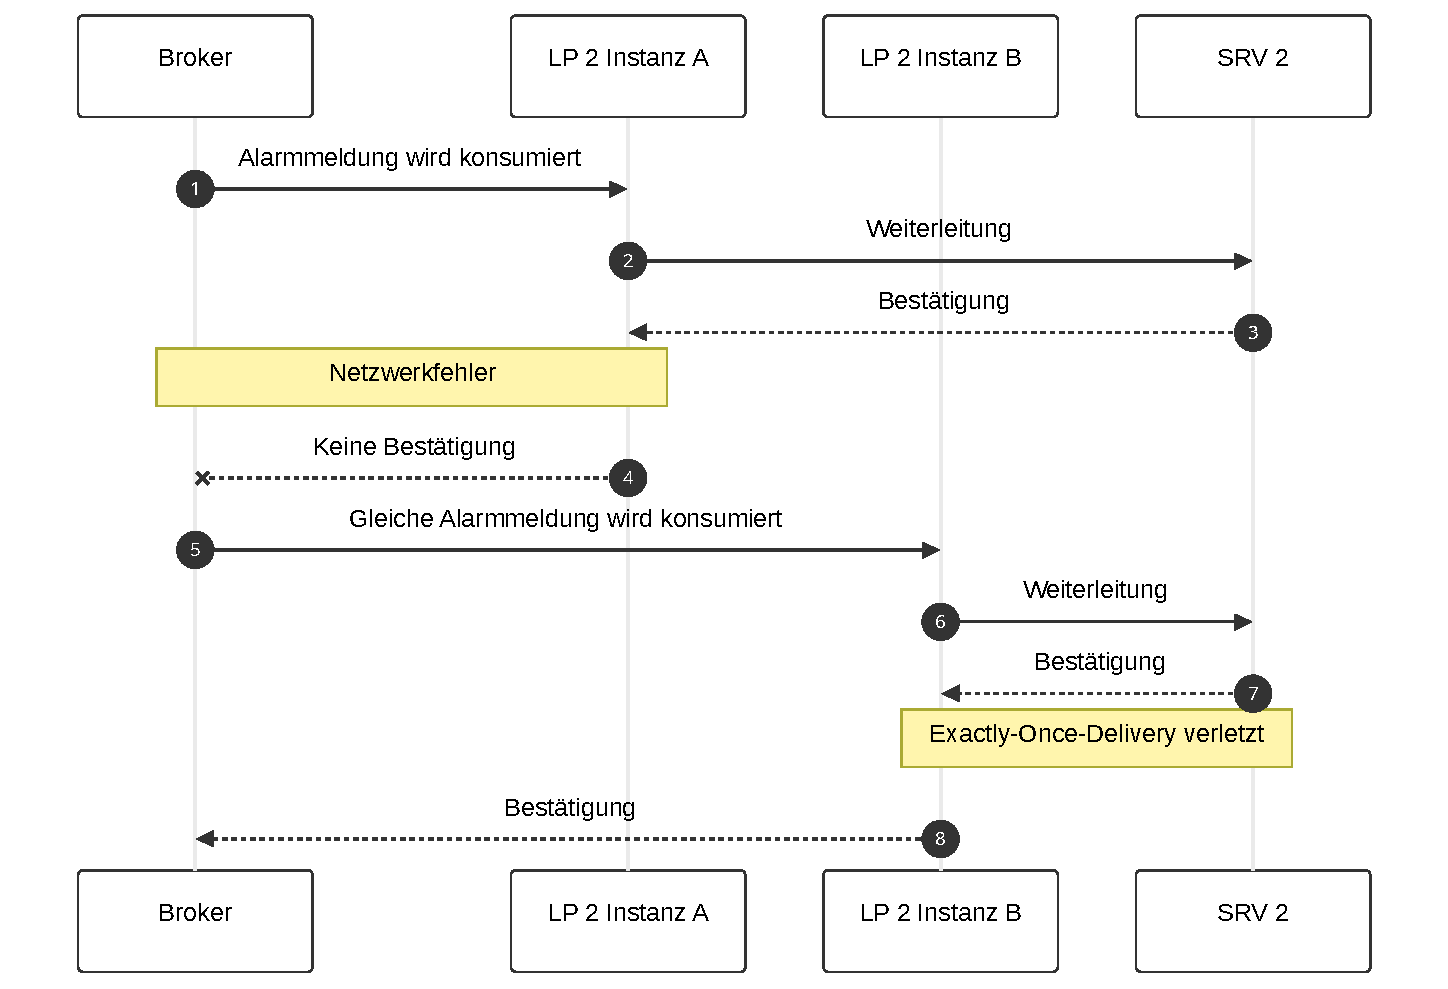
\includegraphics[width=0.479\textwidth]{./img/mermaid/lps_exactly_once_delivery_violation_sequence.pdf}
    \caption{Sequenzdiagramm eines Verarbeitungsablaufs einer Alarmmeldung zur Verletzung der Exactly-Once-Delivery in \acrshort{lps}.}
    \label{fig:lps-exactly-once-delivery-violation-sequence}
\end{figure}

\subsubsection{Verletzung der In-Order-Delivery}
\label{sub-sub:alp-verletzung-iod}

In diesem Abschnitt wird ein Experiment durchgeführt, das gezielt eine Verletzung der \textit{In-Order-Delivery} Garantie in \gls{lps} provoziert. Es wird gezeigt, dass die parallele Verarbeitung von Alarmmeldungen durch mehrere \gls{lptwo}-Instanzen zu einer Verletzung der \textit{In-Order-Delivery} führen kann. Zum Ausführen des Experiments werden die Parameter in Tabelle~\ref{tab:exp-lps-iod-config} ausgewählt. Die quantitativen Parameter $N_{\text{lp~1}}$, $N_{\text{lp~2}}$, $N_{\text{device}}$ und $N_{\text{alarm}}$ werden so gewählt, dass die minimale Anzahl generierter Alarmmeldungen sowie beteiligter Komponenten verwendet wird, mit der eine Verletzung der \textit{In-Order-Delivery} auftreten kann. Die zeitlichen Parameter $I_{\text{alarm}}$ und $T_{\text{max,server}}$ werden so gewählt, dass verschiedene Alarmmeldungen parallel durch mehrere \gls{lptwo}-Instanzen verarbeitet werden und die Wahrscheinlichkeit erhöht wird, dass sie in der falschen Reihenfolge beim \textit{Server-Simulator} ankommen. Da die tatsächliche Verarbeitungszeit zufällig zwischen $T_{\text{min,server}} = 0$\,s und $T_{\text{max,server}}$ bestimmt wird und $T_{\text{max,server}}$ deutlich größer als $I_{\text{alarm}}$ ist, kann die Verarbeitung der zweiten Alarmmeldung vor der ersten abgeschlossen werden, obwohl sie 100\,ms später gesendet wurde. Bei einer festen Verarbeitungszeit ($T_{\text{min,server}} = T_{\text{max,server}}$) wäre dies nicht möglich, da beide Alarmmeldungen gleich lange verarbeitet würden und somit in der Sendereihenfolge beim \textit{Server-Simulator} ankämen. Ursprünglich wurde \textit{HiveMQ CE} in Version \textit{2025.5} als Message Broker verwendet. Jedoch ist die Simulation aufgrund eines ungelösten Bugs~\citep{hivemq_issue_558} in \textit{HiveMQ CE} gescheitert. Der Bug verhindert die parallele Verarbeitung von \gls{mqtt}-Nachrichten durch mehrere Consumer einer einzelnen \textit{Shared Subscription}. Dieser Bug scheint auch in älteren Versionen von \textit{HiveMQ CE} zu existieren~\citep{hivemq_issue_558}. Daher wurde auf \textit{HiveMQ CE} verzichtet und stattdessen \textit{Mosquitto}~\citep{mosquitto} in Version \textit{2.1.2} als Message Broker verwendet. Die Verwendung eines anderen Brokers ist dadurch gerechtfertigt, dass \gls{lps} standardisierte \gls{mqtt}~v5-Features verwendet, die von allen \gls{mqtt}~v5-kompatiblen Brokern unterstützt werden. Außerdem ist dieses Experiment so aufgebaut, dass weder fehlerhafte Verarbeitungen der Alarmmeldungen noch Netzwerkfehler auftreten. Dadurch publizieren die \gls{lptwo}-Instanzen keine Alarmmeldungen auf das Retry-Topic, und das \textit{HiveMQ}-spezifische Plugin des Retry-Mechanismus kommt nicht zum Einsatz.

\begin{table}[H]
    \centering
    \caption{Konfiguration des Experiments zur Verletzung der In-Order-Delivery in \acrshort{lps}.}
    \label{tab:exp-lps-iod-config}
    \begin{tabular}{|l|l|l|}
        \hline
        \textbf{Parameter}      & \textbf{Beschreibung}                  & \textbf{Wert} \\
        \hline
        $N_{\text{lp~1}}$       & Anzahl \gls{lpone}-Instanzen           & 1             \\
        $N_{\text{lp~2}}$       & Anzahl \gls{lptwo}-Instanzen           & 2             \\
        $N_{\text{device}}$     & Anzahl Alarmanlagen                    & 1             \\
        $N_{\text{alarm}}$      & Anzahl Alarmmeldungen pro Alarmanlage  & 2             \\
        $I_{\text{alarm}}$      & Sendeintervall pro Alarmanlage         & 100\,ms       \\
        $T_{\text{min,server}}$ & Minimale Server-Verarbeitungszeit      & 0\,s          \\
        $T_{\text{max,server}}$ & Maximale Server-Verarbeitungszeit      & 5\,s          \\
        $E_{\text{server}}$     & Serverfehlerrate                       & 0{,}0\,\%     \\
        $T_{\text{idle}}$       & Server-Idle-Zeit                       & 5\,s          \\
        $E_{\text{tcp}}$        & \gls{tcp}-Fehlerrate                   & 0{,}0\,\%     \\
        $T_{\text{tcp}}$        & Verbindungsdauer im \gls{tcp}-Proxy    & $\infty$      \\
        $S$                     & Seed des Pseudozufallszahlengenerators & 2             \\
        \hline
    \end{tabular}
\end{table}

Ein Durchlauf gilt als erfolgreich, wenn mindestens eine Alarmmeldung als \textit{Außer Reihenfolge} klassifiziert wird. Als Maß für die Verletzung wird die Außer-Reihenfolge-Rate verwendet, also der Anteil der als \textit{Außer Reihenfolge} klassifizierten Alarmmeldungen an allen eindeutig empfangenen Alarmmeldungen eines Durchlaufs. In allen 59 Durchläufen ist die Außer-Reihenfolge-Rate größer als 0, im Durchschnitt beträgt sie 50{,}0\,\%. Damit kann mit einer Konfidenz von 95\,\% behauptet werden, dass ein Durchlauf mit dem Seed $S = 2$ die Verletzung der \textit{In-Order-Delivery} mit einer Wahrscheinlichkeit von mindestens 95\,\% reproduziert. Die Erklärung dafür ist, dass aufgrund der \textit{Shared Subscription} mehrere \gls{lptwo}-Instanzen Alarmmeldungen parallel verarbeiten. Bei hohen Netzwerklatenzen oder variablen Verarbeitungszeiten der Alarmmeldungen in den nachgelagerten Services kann dies dazu führen, dass Alarmmeldungen in der falschen Reihenfolge beim letzten Service der Verarbeitungskette ankommen. In diesem Experiment ist der letzte Service der Verarbeitungskette der \textit{Server-Simulator}. Im realen \gls{marc}-System ist es \gls{srv}~3, der die Alarmmeldungen in der Datenbank persistiert. Abbildung~\ref{fig:lps-in-order-delivery-violation-sequence} veranschaulicht diese Erklärung als Sequenzdiagramm. Dadurch wird gezeigt, dass \gls{lps} bei variablen Netzwerklatenzen oder variablen Verarbeitungszeiten der Alarmmeldungen in den nachgelagerten Services durch die parallele Verarbeitung von Alarmmeldungen durch mehrere \gls{lptwo}-Instanzen die \textit{In-Order-Delivery} Garantie verletzt.

\begin{figure}[H]
    \centering
    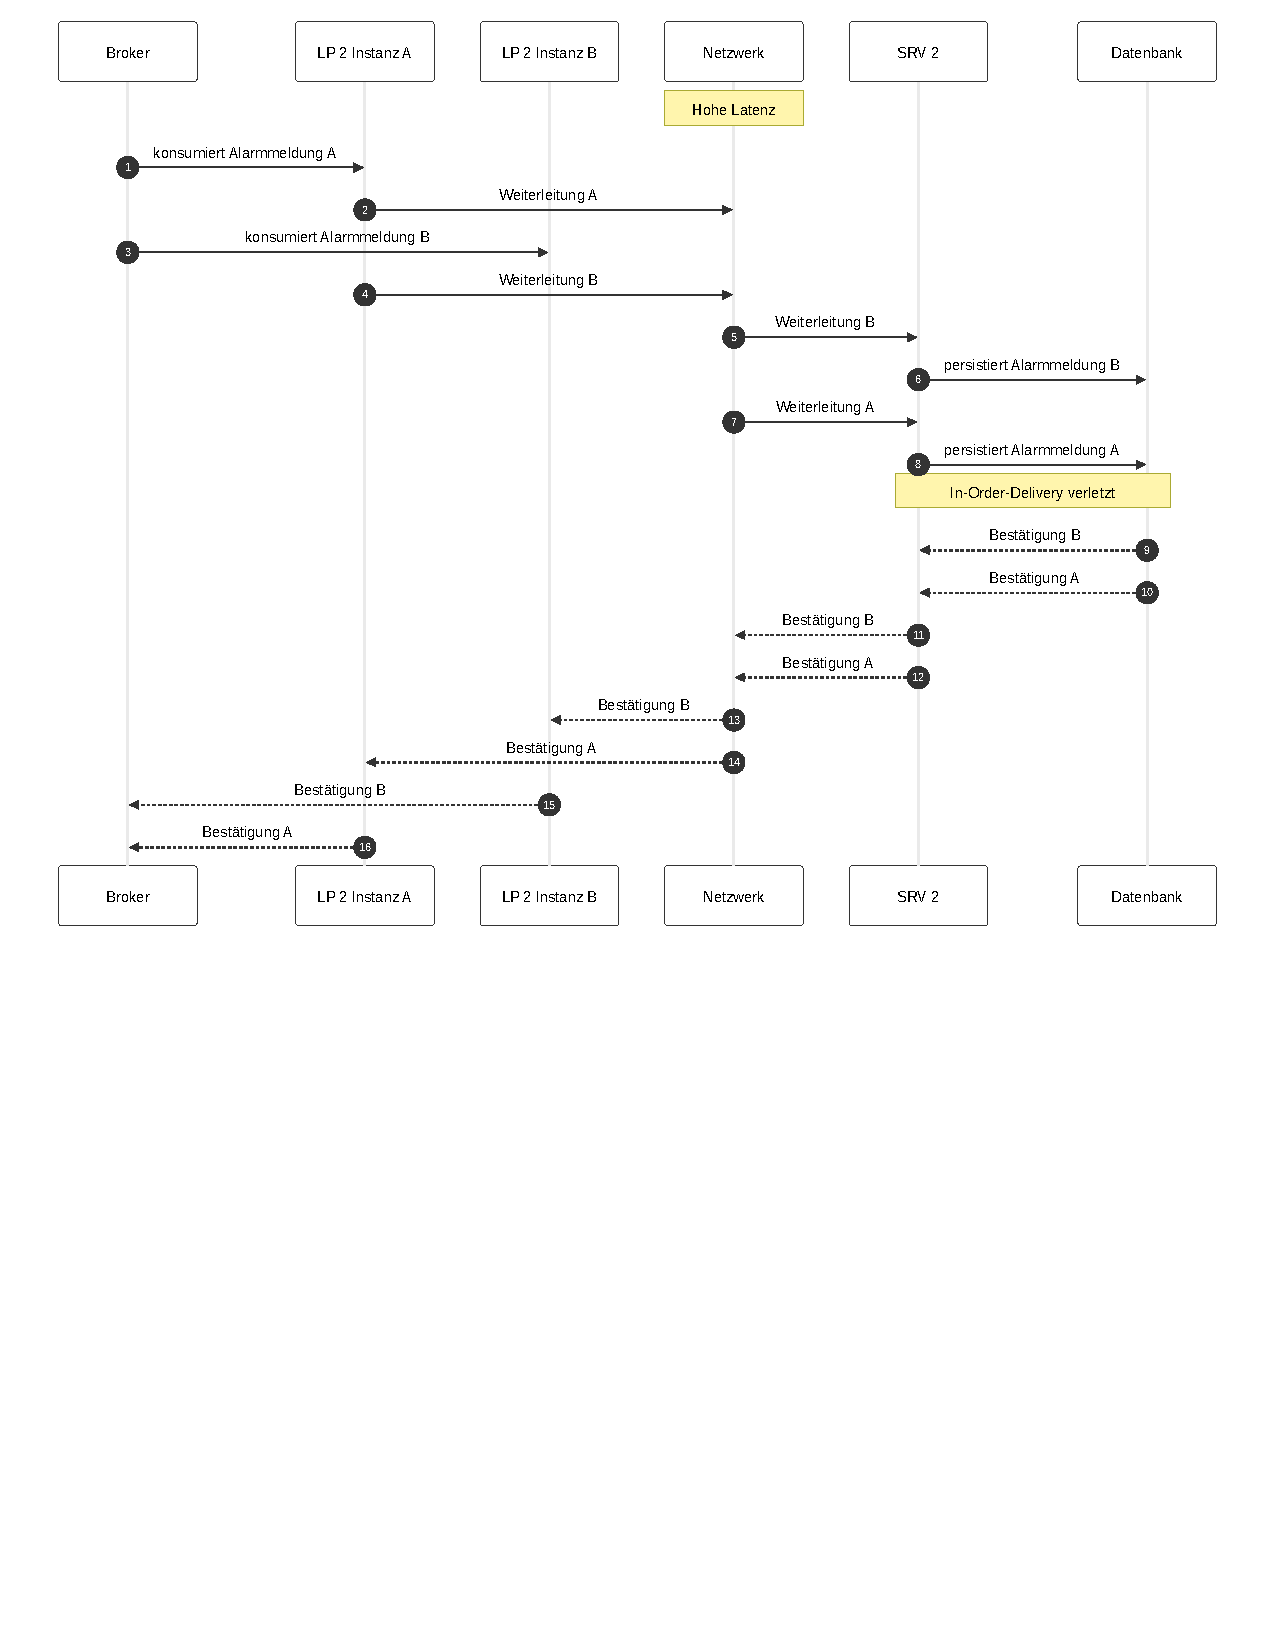
\includegraphics[width=\textwidth]{./img/mermaid/lps_in_order_delivery_violation_sequence.pdf}
    \caption{Sequenzdiagramm eines Verarbeitungsablaufs von Alarmmeldungen zur Verletzung der In-Order-Delivery in \acrshort{lps}.}
    \label{fig:lps-in-order-delivery-violation-sequence}
\end{figure}

Alle Experimente in diesem Abschnitt wurden mithilfe von \textit{Docker Compose}~\citep{docker_compose} durchgeführt und sind anhand von Konfigurationsdateien und der angegebenen Seeds reproduzierbar. Weitere Informationen zum Ausführen der Experimente werden in Abschnitt~\ref{sec:appendix-reproducibility} erläutert. Die Experimente erfolgten auf einem System mit einer \textit{Intel(R) Core(TM) i5-9600K} CPU~\citep{intel_i5_9600k}, 16\,GB \gls{ram} und \textit{Ubuntu} 24.04.4~\citep{ubuntu_24_04}.

\section{Limitationen}
\label{sec:lps-limitationen}

Die Experimente im vorherigen Abschnitt~\ref{sub-sec:lps-experimente} zeigen, dass \gls{lps} die Delivery-Garantien unter bestimmten Bedingungen verletzt. Beim Auftreten von Netzwerkfehlern zwischen \gls{lps}-Komponenten wird die \textit{Exactly-Once-Delivery} Garantie verletzt und bei variablen Netzwerklatenzen oder variablen Verarbeitungszeiten der Alarmmeldungen in den nachgelagerten Services wird die \textit{In-Order-Delivery} Garantie verletzt, wenn mehrere \gls{lptwo}-Instanzen Alarmmeldungen parallel verarbeiten. Eine weitere Limitation von \gls{lps} hat sich beim Durch\-füh\-ren der Experimente indirekt gezeigt. Das entwickelte Retry-Mechanismus Plugin ist vendor-spezifisch und kann nicht auf andere Broker übertragen werden. Dies führt zu einer Abhängigkeit von einem bestimmten Broker, was die Portabilität und Flexibilität des Systems einschränkt. Zusammenfassend ergeben sich folgende Limitationen von \gls{lps}:

\begin{itemize}
    \item Verletzung der \textit{Exactly-Once-Delivery} Garantie.
    \item Verletzung der \textit{In-Order-Delivery} Garantie.
    \item Vendor-Lock-in durch das vendor-spezifische Plugin.
\end{itemize}
